\documentclass[final]{beamer}

\usepackage[scale=1.24,size=a0]{beamerposter} % Use the beamerposter package for laying out the poster

\usetheme{confposter} % Use the confposter theme supplied with this template

% Many more colors are available for use in beamerthemeconfposter.sty
% Modified for Oxford colours by Karl Moritz Hermann

%-----------------------------------------------------------
% Define the column widths and overall poster size
% To set effective sepwid, onecolwid and twocolwid values, first choose how many columns you want and how much separation you want between columns
% In this template, the separation width chosen is 0.024 of the paper width and a 4-column layout
% onecolwid should therefore be (1-(# of columns+1)*sepwid)/# of columns e.g. (1-(4+1)*0.024)/4 = 0.22
% Set twocolwid to be (2*onecolwid)+sepwid = 0.464
% Set threecolwid to be (3*onecolwid)+2*sepwid = 0.708

\newlength{\sepwid}
\newlength{\onecolwid}
\newlength{\twocolwid}
\newlength{\threecolwid}
\setlength{\sepwid}{0.016\paperwidth} % Separation width (white space) between columns
\setlength{\onecolwid}{0.312\paperwidth} % Width of one column
\setlength{\twocolwid}{0.616\paperwidth} % Width of two columns
\setlength{\threecolwid}{0.932\paperwidth} % Width of three columns
\setlength{\topmargin}{-0.5in} % Reduce the top margin size
%-----------------------------------------------------------

\usepackage{graphicx}  % Required for including images
\usepackage{epstopdf}

\usepackage{booktabs} % Top and bottom rules for tables

\usepackage{xspace} % Xspace in commands below
\usepackage{amsmath} %math, align

\usepackage{tikz}
\usetikzlibrary{arrows,positioning,calc,backgrounds,shapes,fit,snakes,mindmap,shadows}
\usepackage{pgfplots}
\pgfplotsset{compat=1.8}

%----------------------------------------------------------------------------------------
%	CUSTOM COMMANDS
%----------------------------------------------------------------------------------------

\newcommand{\modA}{CCAE-A\xspace}
\newcommand{\modB}{CCAE-B\xspace}
\newcommand{\modC}{CCAE-C\xspace}
\newcommand{\modD}{CCAE-D\xspace}

\newcommand{\biCVM}{\textsc{biCVM}\xspace}
\newcommand{\biCVMplus}{\textsc{biCVM+}\xspace}

\newcommand\blocksub[1]{\vspace{0.5em}{\large\color{OxfordBlue}{\textbf{#1}}}\vspace{0.5em}\\}
\newcommand\bbb[1]{{\color{OxfordBlue}{\textbf{#1}}}}

%----------------------------------------------------------------------------------------
%	TITLE SECTION
%----------------------------------------------------------------------------------------

\title{Multilingual Distributed Representations without Word Alignment} % Poster title

\author{Karl Moritz Hermann and Phil Blunsom} % Author(s)

\institute{Department of Computer Science, University of Oxford} % Institution(s)

%----------------------------------------------------------------------------------------

\begin{document}

\addtobeamertemplate{block end}{}{\vspace*{2ex}} % White space under blocks
\addtobeamertemplate{block alerted end}{}{\vspace*{2ex}} % White space under highlighted (alert) blocks

\setlength{\belowcaptionskip}{2ex} % White space under figures
\setlength\belowdisplayshortskip{2ex} % White space under equations

\renewcommand{\arraystretch}{1.2} % Larger spacing among table rows

\begin{frame}[t] % The whole poster is enclosed in one beamer frame
  \begin{columns}[t] % The whole poster consists of three major columns, the second of which is split into two columns twice - the [t] option aligns each column's content to the top
  \begin{column}{\sepwid}\end{column} % Empty spacer column
    \begin{column}{\onecolwid} % The first column
      \begin{alertblock}{TL;DR}
        ~\\
        \textbf{Multilingual Distributed Representations}
        \begin{itemize}
          \item Semantic-transfer across languages
          \item Compositional model means no need for word alignments
          \item Noise-contrastive max-margin approach for joint learning
          \item Approach applicable to any type of compositional vector model
          \item Concise model outperforming state of the art on several tasks
        \end{itemize}
        \vspace{0.5em}
      \end{alertblock}
        ~\\
      \begin{block}{Extending the Distributional Hypothesis}
        ~\\
        The distributional hypothesis is used to learn word representations
        based on the context that these words appear in.
        ~\\
        ~\\
        We extend this hypothesis to learn representations based on the
        \textit{semantic} context of words, and use multilingual data to provide this
        context.
        ~\\
        ~\\
        We use a compositional vector model to transfer semantics at the
        sentence level, thereby preventing bias from noisy alignments and
        capturing the broader semantic context.
        ~\\
        ~\\
      \end{block}

      \begin{block}{The \biCVM Objective Function}
        \textbf{Strongly align representations of semantically equivalent
          sentences $(a,b)$:}
        \begin{equation}
          E_{dist}(a,b) = \left\| f(a) - g(b) \right\|^2\label{eqn:bi-error}
        \end{equation}
        ~\\
        \textbf{Maintain a margin between unaligned sentence pairs $(a,n)$:}
        \begin{equation}
          E_{noise}(a,b,n) = \left[1 + E_{dist}(a,b) - E_{dist}(a,n)\right]_{+}
        \end{equation}
        ~\\
        \textbf{The resulting objective function for a parallel corpus
          $\mathcal{C}_{A,B}$:}
        \begin{equation}
          J(\theta_{bi})=\sum_{(a,b) \in \mathcal{C}_{A,B}} \left( \sum_{i=1}^{k}
            E_{noise}(a,b,n_i)\right) + \frac{\lambda}{2}\|\theta_{bi}\|^2
        \end{equation}
      \end{block}
    \end{column} % End of the first column

  \begin{column}{\sepwid}\end{column} % Empty spacer column

    \begin{column}{\onecolwid} % Column two
      \begin{block}{The \biCVM Model}
        \begin{figure}
          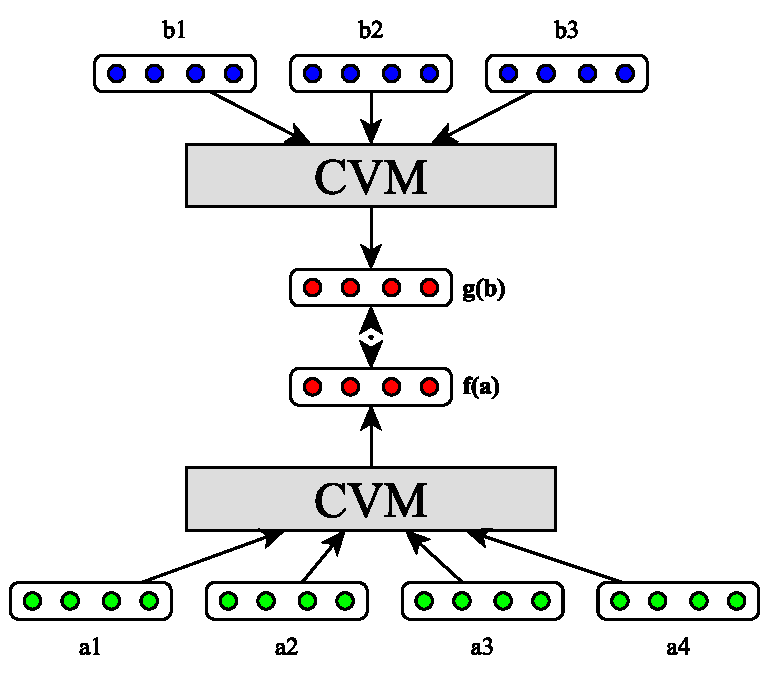
\includegraphics[scale=2.7]{fig3.pdf}
          \caption{Schematic description of \biCVM model applied to two
            sentences $a$ and $b$, using composition vector models $f$ and $g$.}
          \label{fig:ccgrae}
        \end{figure}
      \end{block}

      \begin{block}{Experimental Setup}
        ~\\
    \begin{enumerate}
      \item \textbf{Representation Learning}\\
        We train our model on 500,000 parallel sentences from the Europarl
        corpus (v7, German-English section) using adaptive gradient descent and
        an $L_2$ regularizer.\\
        ~\\
        \biCVMplus is additionally trained on English-French parallel
        data.
        ~\\
        ~\\
      \item \textbf{Classifier training}\\
        Using the trained model, we learn representations for the documents in
        the RCV v2 corpus training data, and then train an averaged perceptron
        to classify these documents by label (4 labels). Settings as in
        Klementiev et al. (2010).
    \end{enumerate}
      \end{block}


    \end{column} % End of column two

  \begin{column}{\sepwid}\end{column} % Empty spacer column

    \begin{column}{\onecolwid} % Column three

      \begin{block}{Cross-Lingual Document Classification}
      The BiCVM models outperform the prior state of the art on a cross-lingual
      document classification task, where a simple classifier is trained using
      data in one language and then evaluated on text from a second language.
  \begin{figure}[t]
    \begin{tikzpicture}
      \begin{axis}[
          height=14cm,
          width=25cm,
          axis x line=bottom,
          axis y line=box,
          % axis lines=left,
          xtick=data, ytick={50,60,...,90},
          enlarge x limits=0.50,
          % enlarge y limits=0.15,
          ymin=45, ymax=87,
          % xmin=2,xmax=5,
          ybar=8pt,
          legend style={at={(0.5,-0.2)}, anchor=north,legend columns=-1,
            draw=none},
          ylabel={F1-Score},
          ylabel near ticks,
          symbolic x coords={en$\rightarrow$de,de$\rightarrow$en},
          nodes near coords,
          nodes near coords align={vertical},
          every node near coord/.append style={font=\small},
          bar width=45pt,
          x=400pt,
          ]
        \addplot[black,fill=black!25]   coordinates {(en$\rightarrow$de,46.8) (de$\rightarrow$en,46.8)};
        \addplot[red,fill=red!25]     coordinates {(en$\rightarrow$de,65.1) (de$\rightarrow$en,68.6)};
        \addplot[teal,fill=teal!25]     coordinates {(en$\rightarrow$de,68.1) (de$\rightarrow$en,67.4)};
        \addplot[brown,fill=brown!25]     coordinates {(en$\rightarrow$de,77.6) (de$\rightarrow$en,71.1)};
        \addplot[blue,fill=blue!75]     coordinates {(en$\rightarrow$de,83.7) (de$\rightarrow$en,71.4)};
        \addplot[purple,fill=purple!75] coordinates {(en$\rightarrow$de,86.2) (de$\rightarrow$en,76.9)};
    \legend{Majority~~,Gloss~~,MT~~,I-Matrix~~,\biCVM~~,\biCVMplus}
      \end{axis}
    \end{tikzpicture}
    \caption{Results on the RCV cross-lingual document classification task.}
  \end{figure}
      \end{block}

      \begin{block}{Qualitative Analysis}
        \begin{figure}
          \fbox{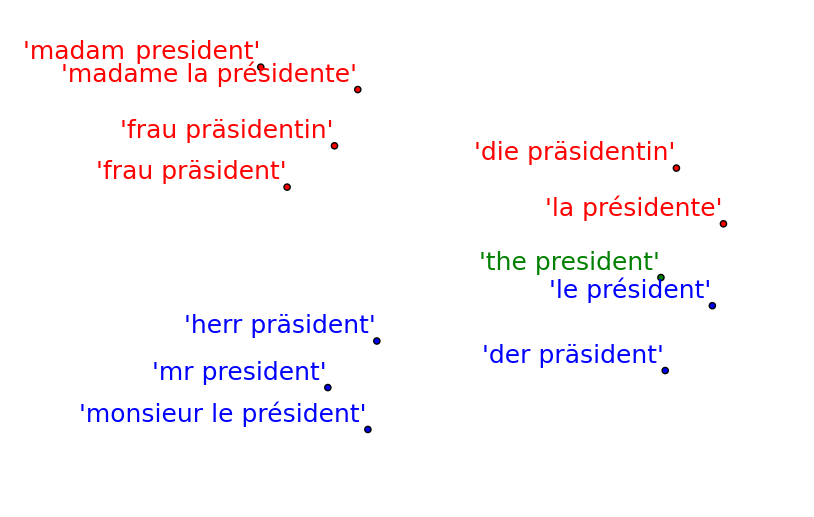
\includegraphics[scale=1.7]{fig4.png}}
          % \vspace{-2em}
          \caption{t-SNE projections from a model trained on two language pairs
            (English-German and English-French). The colours denote gender, with
            green denoting the gender neutral English form.}
          \label{fig:ccgrae}
        \end{figure}
      \end{block}

    \end{column} % End of the fourth column

  \begin{column}{\sepwid}\end{column} % Empty spacer column
  \end{columns} % End of all the columns in the poster
\end{frame} % End of the enclosing frame

\end{document}
